\documentclass{article}
\usepackage{arxiv}

\usepackage[utf8]{inputenc} % allow utf-8 input
\usepackage[T1]{fontenc}  % use 8-bit T1 fonts
\usepackage{hyperref}     % hyperlinks
\usepackage{url}      % simple URL typesetting
\usepackage{booktabs}     % professional-quality tables
\usepackage{amsfonts}     % blackboard math symbols
\usepackage{nicefrac}     % compact symbols for 1/2, etc.
\usepackage{microtype}    % microtypography
\usepackage{graphicx}
\usepackage{xcolor}

\newcommand{\fixme}[1]{{\color{red}\textbf{FIXME:} #1}}
\newcommand{\Eal}[1]{{\color{blue}\textbf{Edward:} #1}}

\definecolor{darkgreen}{RGB}{20,150,50}
\newcommand{\Marjan}[1]{{\color{darkgreen}\textbf{} #1}}
\newcommand{\MS}[1]{{\color{darkgreen}\textbf{Marjan:} #1}}

%%%%% For code listings.
\usepackage{listings}
\lstdefinelanguage{LF}{
  keywords={reaction, preamble, target, reactor, composite, trigger, input, output, new, action, physical, clock, actor, int, main, Main, timer},
  identifierstyle=\color{black},
  sensitive=false,
  comment=[l]{//},
  morecomment=[s]{/*}{*/},
  morestring=[b]',
  morestring=[b]"
}
\definecolor{backcolour}{rgb}{0.95,0.95,0.95}
 
\lstdefinestyle{lfstyle}{
  basicstyle=\ttfamily\footnotesize,
  backgroundcolor=\color{backcolour},   
  keywordstyle=\bfseries,
  breakatwhitespace=false,     
  breaklines=true,         
  captionpos=b,          
  keepspaces=true,         
  numbers=left,          
  numbersep=5pt,
  numberstyle=\tiny,
  showspaces=false,        
  showstringspaces=false,
  showtabs=false,          
  tabsize=2
}
\lstset{language=LF,style=lfstyle}

\title{Verification of Cyberphysical Systems}


\author{
  Marjan Sirjani\thanks{FIXME} \\
  FIXME: Address \\
  \texttt{marjan.sirjani@mdh.se} \\
  %% examples of more authors
   \And
 Edward A. Lee \\
  Department of EECS\\
  FIXME \\
  \texttt{eal@berkeley.edu} \\
}

\begin{document}
\maketitle

\begin{abstract}
FIXME
\end{abstract}


% keywords can be removed
\keywords{First keyword \and Second keyword \and More}


\section{Introduction}

%%%%%%%%%%%%%%%%%%%%%%%%%%%%%%%%%%%%%%
\section{Headings: first level}
\label{sec:headings}

Formal verification is about assuring properties of models.
Whether such properties are also assured in the physical system being modeled
depends on the relationship between the model and 
%that
\Marjan{the}
physical system.
When verifying software, we can often ignore this relationship and rely on the hardware to
faithfully carry out the operations specified by the software.
Hence, when we prove that the software has some property, such as never reaching some undesired state,
we can assume that, with very high probability, the physical system that executes the software will
also have that property.
When verifying cyberphysical systems (CPS), where software reads sensor data and issues commands to physical
actuators, ignoring this relationship is dangerous.
For CPS, verification is ultimately about assuring properties of the physical world
not the software abstraction.

\MS{I am still not sure how CPS is different from reactive systems which by definition interact with their environment, and the environment is (or can be) the physical world. - I think one point of difference with "ordinary" model checking of reactive systems is that we are considering "time" explicitly. Although you say when we talk about state there is always a notion of time, but "ordinary" model checking is not talking about "time" at all, it is talking about transitions (changes to the values of variables of interests). 
Time is somewhere there, but implicitly. Time is there, and a clear reason is that for reactive systems we no more can use predicate logic as the property language, we need to use temporal logic.
Even in temporal logic which is talking about time (it is the logic related to time), we do not have notion of time explicitly, we need TCTL or MLTL to see the "time" explicitly. So, one difference I can see in CPS and reactive systems in general is that we need to take care of time explicitly (and WHY is that?? why time is an intrinsic part of CPS?).

So, here, for CPS we are automatically in the domain of "Timed model checking", or "Verification of Timed Models". In the domain of timed model checking I have to refresh my knowledge, but as far as I know they just talk about "action" transitions and "time" transitions, and they have not talked about this mix of things and did not play with it much. That is why FTTS seems so interesting to me, I think no one looked at it like that. What we are doing here is interesting (never mind novel or not, but I think it is novel too) because we are talking about these things considering "Time". We have these spectrum of equivalency (\url{http://theory.stanford.edu/~rvg/} - \url{http://theory.stanford.edu/~rvg/abstracts.html#19}) talking about all different ways of what we "observe", but it is in the "untimed" world.
We are doing it in the "timed" version. This is what we did in practice in FTTS, but there is so much more to do and to discuss there. I have to read about this, I'll ask Mohammad, he will send me the best stuff.}

Consider a train door with a button that passengers use to open the door \cite{ASYDE-Invited2019Sirjani}.
The software controlling train systems is able to lock the door, disabling the button, while the train is moving.
If we do not know how a passenger's button press is sensed by the software,
and how the door gets locked in response to a software command, then it will do
little good to prove that the software never enters a state where it thinks the door is
unlocked while the train is moving.

To illustrate this point, consider the sketch of an implementation in Figure \ref{fig:lf}
of a highly simplified version of such train controller software.
This implementation is written using Lingua Franca (LF) \cite{FIXME}, a coordination language
designed for safety-critical real-time systems.
In this use, the code shown in the figure gets translated into C code that can run on a train's microcontrollers.

\begin{figure}[bt]
\centering
\begin{minipage}{0.50\linewidth}
\begin{lstlisting}[language=LF]
target C;
reactor Button {
  output open:bool;
  physical action button:bool;
  initialize {=
    ... Set up sensing.
  =}
  reaction(button)->open {=
    set(open, true);
  =}
}
reactor Door {
  input lock:bool;
  input open:bool;
  state locked:bool(false);
  reaction(lock) {=
    if (lock) {
      self->is_open = false;
    }
    self->locked = lock;
  =}
  reaction(open) {=
    if (!self->locked){
      ... Actuate.
    }     
  =}
}
\end{lstlisting}
\end{minipage}%
\begin{minipage}{0.45\linewidth}
\begin{lstlisting}[language=LF,firstnumber=28]
reactor Train {
  output lock:bool;
  state moving:bool(false);
  physical action stopped:bool;
  initialize {=
    ... Set up sensing.
  =}
  reaction(stopped) -> lock {=
    if (stopped) {
      self->moving = false;
      set(lock, false);
    } else {
      self->moving = true;
      set(lock, true);
    }
  =}
}
reactor Main {
  button = new Button();
  door = new Door();
  train = new Train();
  button.open -> door.open;
  train.lock -> door.lock;
}
  
  
.
\end{lstlisting}
\end{minipage}%
\caption{Lingua Franca code for the train example.
\label{fig:lf}}
\end{figure}

\begin{figure}[b]
  \centering
  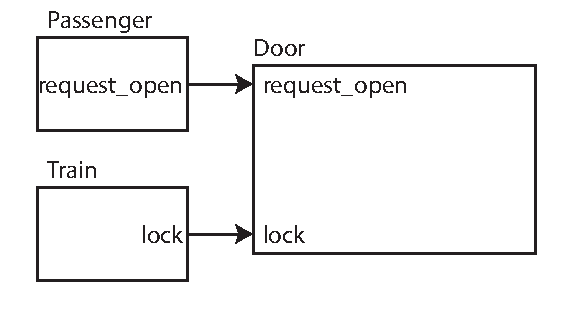
\includegraphics[width=8cm]{DoorControllerSimple.pdf}
  \caption{Sample figure caption.}
  \label{fig:DoorControllerSimple}
\end{figure}

The structure of the code is illustrated in Figure \ref{fig:DoorControllerSimple}.
It consists of three components called ``reactors,'' instances of the reactor classes
Button, Door, and Train. The Main reactor (starting on line 39) instantiates and connects these
components so that the button and the train each send messages to the door.
These components could be implemented on a single core, on multiple cores, or on
separate processors connected via a network.

Let's focus first on the interaction between these components and the physical world.
The Button reactor class defines a \textbf{physical action} named ``button'' (line 4), which in Lingua Franca is an event
that is triggered by something outside the software system and is then assigned a logical timestamp
that approximates the physical time at which that something occurred in the physical world.
In practice, in the \textbf{initialize} block of code (starting on line 5),
(FIXME: There is no such thing in LF)
the reactor could set
up an interrupt service routine (ISR) to be invoked whenever a passenger pushes the button on the door.
The ISR would call an LF function \textbf{schedule} to trigger the action and assign it a timestamp.
The \textbf{reaction} to the button action (starting on line 8) will be invoked when logical time reaches
the assigned timestamp.
This reaction sets the output named ``open'' to the Boolean value true.
Since that output is connected to the input named ''open'' of the door component (line 49),
this results in a message to the door component at the logical time of the timestamp.

The train component similarly has a physical action named ``stopped,''
which is similarly triggered by sensors when the train stops at a station or
begins moving from the station (with Boolean values true and false respectively).
In addition, it has a state variable named ``moving'' that has value true when the train is moving
and false when the train is stopped.
When the train stops or begins moving, this software component sends a message to the
door component (lines 38, 41, and 50).

The door component has a state variable named ``locked'' (line 15) that changes value  when it receives a message
on its ``lock'' input port (lines 13 and 20).
It uses this state variable to guard the opening of the door (line 23).
The actual opening of the door is performed by some I/O mechanism such as writing to a memory-mapped
register (line 24).

For this simple system, the safety property of interest is that the door be locked while the train is moving.
This can be posed as a formal verification problem, where the goal is to prove this property.
To do so, however, we need a model.
And how to construct the ``right'' model proves astonishingly subtle,
even for such a trivial example.
Let us examine the problem.

In the program shown in Figure \ref{fig:lf}, the door and train components
have state variables, and we can attempt to verify that the door is never in the unlocked
state while the train is in the moving state.
Depending on how the physical interfaces are realized, however,
this may or may not align with the physical world.
So while it is not enough to verify that the software does not reach some undesired state,
that's all we can do with the information provided.

With such a trivial example, it seems that it should be easy to determine whether the undesired
state can ever be reached.
Unfortunately, even in such a simple case, there are subtleties.
What if the door component and the train component are executing on two different microprocessors
separated by a network?
What does it mean, in this case, for the two to simultaneously be in some state?
We may naively assume a Newtonian model of time and talk about the state of the microprocessors at
some instant in time, but the actual physical realization has no such instants.
The model that defines the execution of software talks about sequences of steps, not
instants in Newtonian time.
Moreover, no physical measurements of time can identify these simultaneous instants at the two
separate microprocessors because the very notion of simultaneity is ill defined.\footnote{The theory
of relativity tells us that whether two physically separated events are simultaneous depends on the observer.}
In order to verify the system, we need a clearer model.

Most of the most successful verification techniques are based on transition systems \cite{FIXME}.\footnote{FIXME: Cite 2006 FORMATS paper.
That paper argued for replacing semantic models based on state and state transition systems with fixed point theories,
but we show here that we do not need to give up the notion of state and can consequently leverage
advances in model checking technology.
}
A transition system models a process as a sequence of discrete state changes.
The challenge, however, is that the notion of ``state'' is unclear.
The state of a system is the particular condition that the system is in at a specific time.
But this requires a notion of time, and for a distributed systems, a notion of simultaneity.
Physics alone cannot provide these notions.
We have to instead bind these notions to the semantics of the programming language.

Lingua Franca includes in its semantics a notion of logical time.
The messages exchanged between components have timestamps drawn from a discrete, totally ordered model of time.
Any two messages with the same timestamp are logically simultaneous.
At a logical time where there is at least one message in the system,
components react to this message, possibly producing more messages at the same logical time
and causing other components to react as well.
As a consequence, the execution of a Lingua Franca program can be viewed as a sequence
of discrete state transitions, where at a sequence of distinct logical times,
the entire system changes state.
Under such a \textbf{logical-time-based semantics}, it is easy to verify that the LF program
in Figure \ref{fig:lf} never reaches the undesired state.

To perform such verification automatically, we need to build a state-transition model
of the program, as shown in Figure \ref{fig:logicaltimebased}.
In the initial state, indicated by the dangling arrow, the door is unlocked and the train
is not moving.
At each logical time, this state machine will react by nondeterministically either
remaining in the same state (indicated by the self-loop transition) or changing to the state
where the door is locked and the train is moving
(the gaurds on both transitions are ``true,'' indicating that both are enabled).
Once the machine is in the new state, at subsequent logical times,
it will similarly nondeterministically remain in the same
state or transition to initial state.

NOTE: All semantics that uses a transition system is "time based" so calling the semantics "time based" is meaningless. Hence I changed the name to "logical time based".

\begin{figure}[b]
  \centering
  \includegraphics[width=5cm]{LogicalTimeBased.pdf}
  \caption{A transition system for the logical-time-based semantics for the program in Figure \ref{fig:lf}.
  \label{fig:logicaltimebased}}
\end{figure}

The astute reader may be puzzled about how this transition system models the program
in Figure \ref{fig:lf}. In that program, it looks as if the train transitions first to moving,
emitting the lock = true message, and only then does the door react by changing its state to
locked = true. Doesn't this create a transient situation where the train is moving
and the door is unlocked?

The semantics of Lingua Franca is rooted in the fixed-point semantics of synchronous languages
\cite{FIXME}. The train and door components can be modeled as concurrent state machines
as shown in Figure \ref{fig:logicaltimebasedconcurrent}, following the style developed,
for example, in \cite{LeeSeshia:11:EmbeddedSystems}, which is based on Statecharts \cite{Harel:87:Statecharts}
but with a rigorous synchronous semantics.
A vertical bar separates the two concurrent components, the ``train'' and ``door.''
The train component nondeterministically emits the signal lock = true, \Marjan{nondeterministically? I thought in our model-time based transition system we have "time-triggered events" on the transitions as the lables } which causes the door
component to transition to locked = true.
This occurs, however, logically \emph{simultaneously and instantaneously}.
The two machine transition together.
Formally, what transition is taken and what signals are emitted is defined
by a unique fixed point of a monotonic function in a complete partial order \cite{FIXME}.
Every correct implementation of this semantics must behave exactly as if these state transitions
are simultaneous such that no observer can detect the transient intermediate
state where the train is moving and the door is unlocked.
In effect, the transition system of Figure \ref{fig:logicaltimebased} defines
the semantics of the concurrent state machines of Figure \ref{fig:logicaltimebasedconcurrent},
which in turn define the semantics of the program in Figure \ref{fig:lf}.

\begin{figure}[b]
  \centering
  \includegraphics[width=9cm]{LogicalTimeBasedConcurrent.pdf}
  \caption{A concurrent transition system for the logical-time-based semantics for the program in Figure \ref{fig:lf}. \Marjan{ I think in a logical-time-based transition system we need to see the some t on the transition. Which one is nicer? Logical-time-based or model-time-based?}}
  \label{fig:logicaltimebasedconcurrent}
\end{figure}

This approach to verification is logically defensible because it accurately and correctly
models the semantics of the program.
But the astute reader should still be nervous.
What if the train component and the door component are realized on distinct microprocessors
connected over a network? Won't there be a physical time delay between when the train
begins moving and the door gets locked, even if there is no logical time delay?
Doesn't this mean that the transient state is real and should be modeled?
\Marjan{This thesis: http://www.lfcs.inf.ed.ac.uk/reports/88/ECS-LFCS-88-51/ECS-LFCS-88-51.pdf is talking about similar things (in different way I guess), it would make our paper nicer if we make the connection, I'll see what I can do.}


Not necessarily.  PLC style.

FIXME: Unorganized notes below.

We need to recognize that software has side effects in the physical world.
A piece of software unlocks the door (through some actuation), and another piece of software opens the door
(reacting to sensor input and then actuating).
If we understand how sensing and actuation is done, then it may be sufficient to verify the software.

In principle, we can apply model checking \cite{FIXME} to check to see whether the software enters some
state where it has opened the door (through actuation, a side effect) and the train is moving (also through
actuation).
Model checking is based on modeling the software execution as a sequence of state transitions.
There are a number of challenges with building such a model.

First, we have to clearly define what we mean by the state of the software system.
This can be especially difficult in a distributed system or in a software system that executes in parallel,
such as on a multicore.
In particular, it will not work to just define the state of the software as the valuation of all its variables
because such a valuation has to at some \emph{time}, and a distributed system may have no coherent notion
of time.

This problem is not new.
The verification community has dealt with this problem for decades
and very thoughtful debates have occurred over the best way to deal with the problem.
For example, one such debate is over the use of ``interleaving semantics'' vs. ``true concurrency'' \cite{FIXME}.


FIXME: Describe the verification problem for the DoorControllerSimple example.
To perform model checking, we have to model the problem as a transition system.
One possible way of doing that is to model each reaction of the LF program as an atomic transition between states.
With this choice, in general, a LF program will be modeled by a nondeterministic transition system because
there is flexibility in the order in which reactions are invoked (and in whether they are invoked in parallel).
In a way, this is unfortunate, because one of the key strengths of LF is that provided a globally
determinsitic model of computation. Nevertheless, by building such a model, we obtain a transition
system that can be analyzed with well-established model checking tools.

Describe the translation to Rebeca and the use of Afra to expose a potential violation of the safety condition.
Rebeca is a language for building models of CPS, whereas LF is a language for implementing CPS.
A Rebeca model, in principle, has no side effects in the physical world, but rather models
side effects of software components interacting the physical world.
The map and the territory.
Ultimately, we can only verify a map.
But we want to draw conclusions about the territory.

The violation condition is a transient state in that it exists only during a logically instantaneous action,
the computation of all reactions at a logical time.
However, if the reactions have side effects in the physical world, then such a transient state could
in fact last for some non-zero physical time.
This is why, when performing verification of CPS, it is essential to understand how sensing and
actuation is done.

For example, in PLCs, the most widely used programming frameworks for industrial automation \cite{Stanadard},
computations are logically periodic, sensing is done at the beginning of a logical instant before
any computation is done at that instant, and actuation is done after the end of \emph{all} computation
at that logical instant, and hence transient states in the software \emph{cannot} effect the physical world.

An implementation of Lingua Franca could, in principle, do the same thing.
If it restricts all physical I/O to occur between logical time instants, then the transient violating
state found by model checking is not a problem.

Names: Event based, time based, fine grained, PLC style?

If we have such an implementation of LF (FIXME: Name this), then we should construct a different transition system
model of the program for the purposes of model checking.
One way to do that is to define a transition as the entirety of all computation at a logical time instant.
The change of state of the system enacted by this entirety can be modeled as a fixed point
of a monotonic function, using the principles of synchronous languages \cite{FIXME}.

If we do not have such an implementation, and each reaction can have side effects, then the model
we built with Rebeca is a more reasonable model.
However, even that will not be perfect, because it assumes that reactions are atomic.
In a physical realization, reactions will take time to execute, and if they are executing in parallel,
then the ordering of their side effects could become nondeterministic.
This nondeterminism is not captured in the Rebeca model.

Assuming we do not have a (FIXME: Name this) implementation, then the violation exposed by Afra is real
and must be fixed. One way to fix it is with the LF code shown in Figure FIXME, sketched in
Figure \ref{fig:DoorControllerSimpleFixed}.
This program realizes a handshake that ensures that the train does not begin moving until
it has received confirmation that the door has been locked.
If we do have the (FIXME: Name this) implementation, then such a handshake need not be included
in the LF program because, in effect, the required handshake is provided by the implementation of LF.
Thus, the (FIXME: Name this) implementation does more work so that the programmer can do less.

In \cite{other paper}, reactions are assumed to be ``isolated,'' meaning that reactions do not
internally have side effects, and that any side effects in the physical world are actuated between
reactions. However, this has a cost. Parallel execution becomes much more restricted because,
in order to actuate, we have to ensure that \emph{no reaction} is currently executing.
This implies a barrier synchronization each time actuation is done.

NOTE: We could prototype the (FIXME: Name this) implementation easily by using "printf" as the
one and only side effect, standing in for all actuation. We would provide another implementation
of printf that collects all the things to be printed during a logical instant and then
prints them all at once, making it clear that they are logically simultaneous.

Model Checking Lingua Franca
- Formal Semantics of Lingua Franca

Side effects and true concurrency.
Example: printf. Consider two reactions with no dependency on one another.
Each reaction uses multiple printf calls to print information while it executes.
Assume a semantics where state transitions occur on atomic invocations of reactions.
In an interleaving concurrency model, all the print statements of one reaction will precede all
the print statements of the other.
In a true concurrency model, the print statements can be arbitrarily interleaved.


\subsection{Constraints of Interleaving Semantics}

For interleaving semantics (with "atomic" executions, "coarse grain", "reaction level model"???)
to correctly describe parallel executions of reactions with side effects
that affect the same physical object, there is constraint. No reaction can have more than one side effect
on that object. This constraint has been previously observed by the Rebeca team FIXME:citation?Masters thesis?,
where such side effects
are modeled by sending messages to a Rebec that models the physical object being affected.
For the interleaving semantics to correctly model parallel execution, there is a constraint
in timed Rebeca that no two messages with same timestamp can be sent from the same Rebec to same other Rebec.
This is equivalent, in some sense, to the Lingua Franca model, which does not queue messages that are
sent to the same port at a given logical time, but instead overwrites any previous message,
replacing its value with a new one at that logical time.

Examples of Lingua Franca

Differences with Rebeca

Verification

Semantics 

\Marjan{What's the difference between reactive (interactive concurrent systems) in general and CPS?
-- Reactive systems have interaction with environment. What is the difference that causes the differences we are talking about?}

\begin{figure}[b]
  \centering
  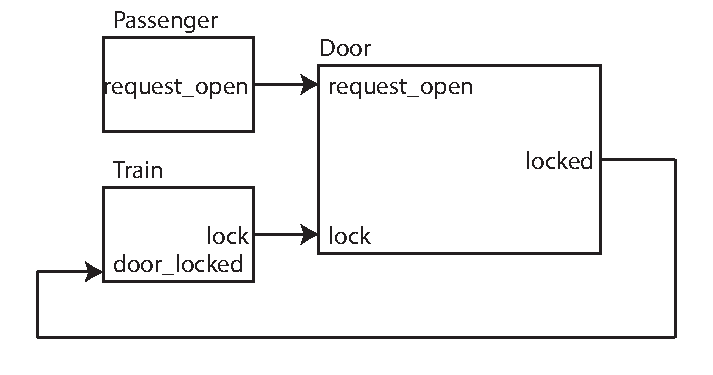
\includegraphics[width=10cm]{DoorControllerSimpleFixed.pdf}
  \caption{Sample figure caption.}
  \label{fig:DoorControllerSimpleFixed}
\end{figure}

\bibliographystyle{unsrt}  
\bibliography{references}

\end{document}
